
\chapter{Development of the network model}\label{paper1}

\section{Introduction}
In order to simulate the propagation, control and vaccination strategies for VPH infections and associated diseases it is necessary to develop a realistic sexual network model capturing the general statistical features of contacts among individuals.

As it is well-known, network modelling is the current approach in mathematical epidemiology because, in contrast with traditional methods based upon systems of differential equations, it allows for a description of infections in terms of contacts among individuals, as it happens in real life, as well as an analysis of the spreading of the disease depending upon the distribution of those contacts or the incidence of vaccination in particular subjects, its clinical history, etc.

In order to understand the evolution of the HPV disease we need a reliable model of the underlying social network in which the pandemic builds up. Individuals who change partners or have several partners simultaneously, are the hubs favoring the spread of sexually transmitted diseases (STI). The distribution of degrees of the nodes in the network and the average path from an infected individual to a susceptible one, are important parameters controlling the final extension of a new STI in a population and the speed of its spread. However, most models are based on some assumptions, which could not be valid for certain populations. Some studies claimed that the web of human sexual contacts is a scale-free network characterized by a power-law distribution for the number of individuals with a certain degree of connectivity, k: $P(k)\propto1/k^\alpha$  with a value of k in the range $2 \textless k \textless 3$, and slightly smaller for males than for females.

Although P(k) provides some valuable information about the network, it is not a sufficient prescription on how to build it for a given population size.
Moreover, a power-law distribution of contacts could not be representative of some populations, or could vary from country to country.

To avoid the shortcomings of these theoretical approaches we have started with real statistical data for Spain and, by applying concepts of network theory to be described below, we have been able to develop network models for populations of 1,000,000 individuals with a distribution of sexual partners among them characterized by the data from surveys of the National Institute of Statistics in Spain (Encuesta de salud y h\'abitos sexuales 2003. \url{http://www.ine.es}).

From previous works we know that populations around 1,000,000 individuals are necessary to sustain pandemics with low prevalence such as Respiratory Syncytial Virus or VPH (See J. Villanueva-Oller et al., Epidemic Random Network Simulations in a Distributed Computing Environment, Abstract \& Applied Analysis, 2013, ID462801). 

\section{Data}
The Community of Valencia is an autonomous region of Spain. It is located in the central and south-eastern side of the Iberian Peninsula. The region is divided into three provinces: Alicante, Castell\'on and Valencia with a total population of 5.1 million inhabitants.

From the statistical data for Valencia (Valentian Institute of Statistics, \url{http://ww.ive.es}) we obtain that 50.71\% of Valencian people with ages between 14-65 years old are male. 

According to the age-groups relevant for VPH modelling we have found that: 25.22 \% of males are aged 14-29, 25.23 \% are aged 30-39 and 49.55 \% are aged 40-65. In a similar way, 24.87 \% of females are aged 14-29, 23.99 \% are aged 30-39, and 51.14 \% are aged 40-65. Following this procedure, we can obtain the percentage of males and females per age inside their corresponding groups. This will be useful to distribute the nodes of a network demographically. In the following, we will use this data to assign ages to the nodes in the network according to the population histogram in Valencia.

The corresponding histograms are shown in Figs. \ref{data1} (men), \ref{data2} (women) and \ref{demog} (both):

\begin{figure}[ht]
	\centering
	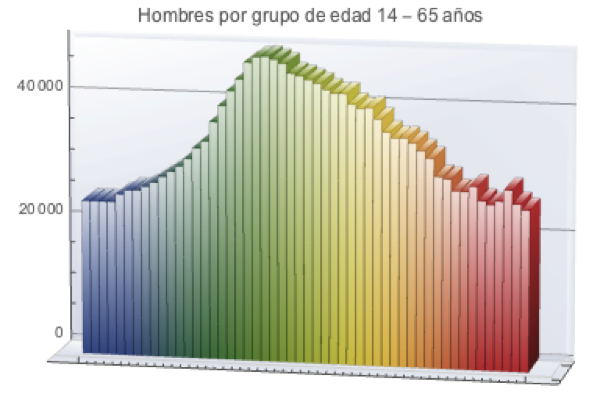
\includegraphics[scale=0.7]{IMG/data1.png}
	\caption{Histogram for the population of men in Valencia (Spain). The range is 14-65 years old.}
	\label{data1}
\end{figure} 

\begin{figure}[ht]
	\centering
	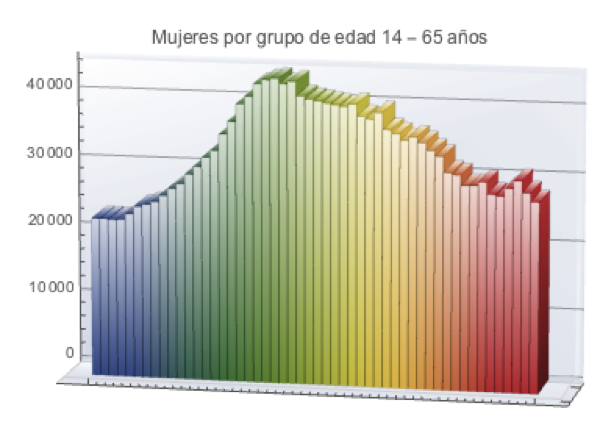
\includegraphics[scale=0.7]{IMG/data2.png}
	\caption{The same as Fig. \ref{data1} but for women.}
	\label{data2}
\end{figure} 

\begin{figure}[ht]
	\centering
	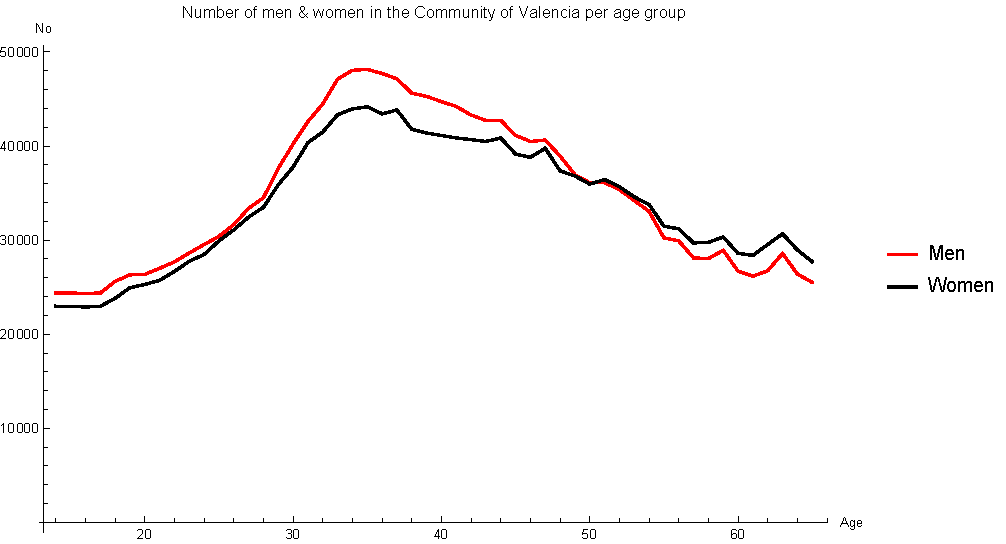
\includegraphics[scale=0.7]{demog.pdf}
	\caption{Number of men and woman in the Community of Valencia per age (year 2013) for both.}
	\label{demog}
\end{figure}

Concerning the sexual behavior the only relevant data for the linking of the network is the number of lifetime sexual partner networks, i. e., the number of sexual partners that an individual have had throughout his/her life until a given age. This is a cumulative historical data that will help us to build a network of lifetime sexual partners (LSP network) but, due to the lack of data on the duration of those relationships and the moment in life in which they occurred, it will be insufficient to ascertain the dynamical aspects of the network and its evolution with time. Nevertheless, we have found that LSPs are a useful tool to study the probability of individuals to contract the infection throughout their lives and the transition to the different stages of the disease. Moreover, LSP capture the essential feature of network modelling consisting of the enhancement of the community effect when people with high number of connections (the hubs of the network) are targeted by vaccination strategies.

In our network we have also considered the homosexual population and the possible contacts of homosexual men with women is some moment in their lives. This is a key issue in the network because it determines the propagation of the VPH infection from the homosexual subpopulation to the whole heterosexual one and vice versa. We have not considered lesbians because the impact of VPH transmission in this subgroup is far smaller.

Lifetime sexual partners for a heterosexual individual (LSP) is obtained from the Health and Sexual Habits Survey 2003, as listed in the table in terms of the age-group. Notice that we do not have more recent information on this topic.

\begin{figure}[ht]
	\centering
	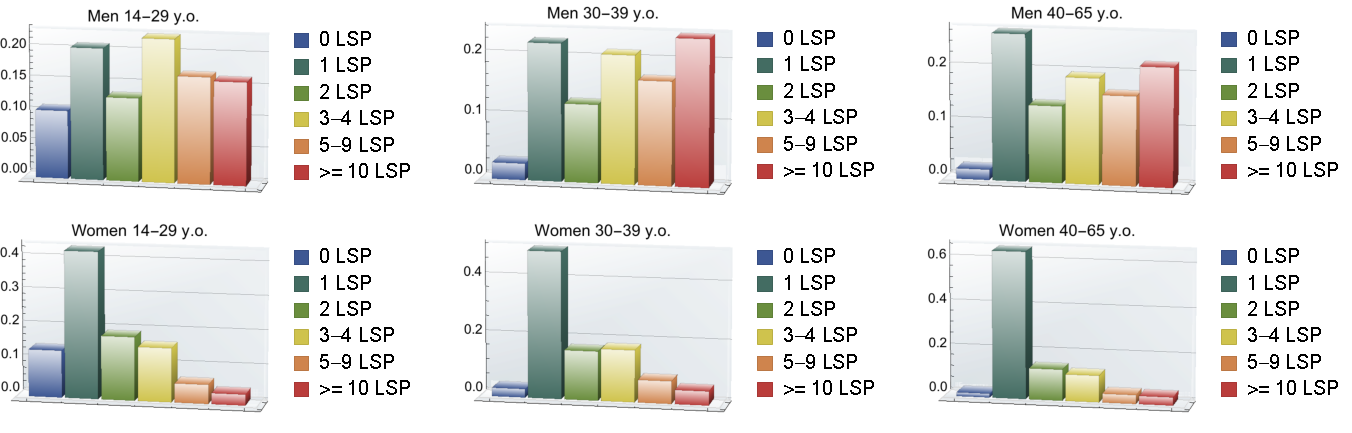
\includegraphics[scale=0.7]{lsp.pdf}
	\caption{Number of lifetime sexual partners (LSP) for men and woman per age group in Spain (year 2003). The age groups are 14-29, 30-39 and 40-65.}
	\label{lsp}
\end{figure}

We now summarize some general features of the distribution of contacts: 

\begin{itemize}
	\item The percentage of males and females with no partners is very similar in each age-group.

	\item The proportion of women with only a partner is, approximately,
the double than men with only one partner. 

	\item The percentage of men with two or more partners is always larger than that of women except for women in the age-groups 14-29, and 30-39 in the case of two partners.

	\item The asymmetry in the behavior of males and females should be taken into account in the construction of the network.
\end{itemize}

This male-female asymmetry is the main challenge in building a realistic LSP network because more sophisticated methods than the simple random assignment of contacts must be used.

The situation for the homosexual population is different because the average number of sexual partners was estimated in 39 regardless of age, in a study by Durex but this number increased with age with a peak of 59 in the 40-49 age-group (Estudio de conducta sexual entre homosexuales, Durex, 26 de junio de 2002).  As we have not to distinguish among the sexes as in the case of the heterosexual subnetwork this case will be treated with standard random network construction.

A difficulty arises because we have little information about the number of sexual contacts with women for the homosexual subpopulation. In a personal communication by M. D\'{\i}az Sanchis (Institut Catal\`{a} d'Oncologia, IDIBELL) we are informed that almost all homosexual men has, sometime in their lives, had a woman partner.  Consequently, we have simulated these connections by assigning a contact to every man in the homosexual subpopulation with a heterosexual woman with 5 partners or more. This is done according to the assortativity principle to be described in the next section.
